% Chapter Template

\chapter{Sensory Redundancy: Are two heads better than one?} % Main chapter title

\label{Chapter4} % Change X to a consecutive number; for referencing this chapter elsewhere, use \ref{ChapterX}

\lhead{Chapter 4. \emph{Sensory Redundancy: Are two heads better than one?}} % Change X to a consecutive number; this is for the header on each page - perhaps a shortened title

%----------------------------------------------------------------------------------------
%	SECTION 1
%----------------------------------------------------------------------------------------

\section{Why have one sensor when two are better?}
A key part of the human experience is that it is multisensory. In \cite{barsalou2008grounded}, Lawrence Barsalou speaks about how multisensory processing aids human cognition in a number of ways. Firstly, multisensory information aids in the classification of experiences by providing additional and complimentary information that is not accounted for in only a single modality. 

The Mcgurk effect \cite{mcgurk1976hearing} demonstrates how the visual stimuli of lip reading affects the classification of heard sounds. Whilst this effect can lead to incorrect classifications when misaligned data is provided e.g. utterances of the syllable [ba] dubbed on to lip movements for [ga], lead to normal adults hearing [da]; in normal circumstances i.e. when two people are speaking to one and other, lip reading aids in classifying heard sounds \cite{ma2009lip}. This is particularly importnant in noisy environments, which leads to another of Barsalou's ideas about multisensory processing: information redundancy.

The reason that lip reading can aid hearing in noisy evironments is that it provides an additional vector along which the human brain can reconstruct missing information. I.e. when something is mis-heard due to background noise, the visual information gained from looking at the face of the speaker can be used to reconstruct their utterance.

The ability to reconstruct missing data from a secondary modality has not only been seen in humans \cite{ma2009lip, samuel1997lexical} but has been demonstrated in computational modals for example, Ngiam et al.\cite{ngiam2011multimodal}.

In this chapter I will explore these two ideas, improved classification and reconstruction of missing information, through the use of neural networks.

\subsection{Aims}
This chapter contains two experiments. The first experiment looks at whether having access to a second modality improves classification accuracy over the baseline accuracy of classification of either of the two individual modalities.

The second experiment looks at classification accuracy using bimodal data as well as how well a missing data can be reconstructed from a secondary modality.

\section{MIRFLICKR-25000}
\label{sec:flikr}
\subsection{Dataset Description}
MIRFLICKR-25000 (Flikr25K) is an image classification dataset containing 25,000 images as well as textual tags. Images were collected from the social media site, Flikr.com along with user provided tags. \footnote{A full description of the datset can be found at https://press.liacs.nl/mirflickr/.}

On average images have 8.94 tags and there are xx unique tags. Each image falls into 1 of 24 classes. 
The dataset is not balanced as there are different numbers of images per class as seen in figure \ref{fig:flikr_freq} and table \ref{tab:flikr_freq}. This makes classifying the dataset difficult as there will be a large bias towards classes which occur more frequently. For example, the most common class ``structures'' occurs 9992 times compared to the least common class ``baby'' which only occurs 116 times, making ``structures'' more than 86 times as likely to occur than ``baby''.

\begin{figure}
	\begin{center}
		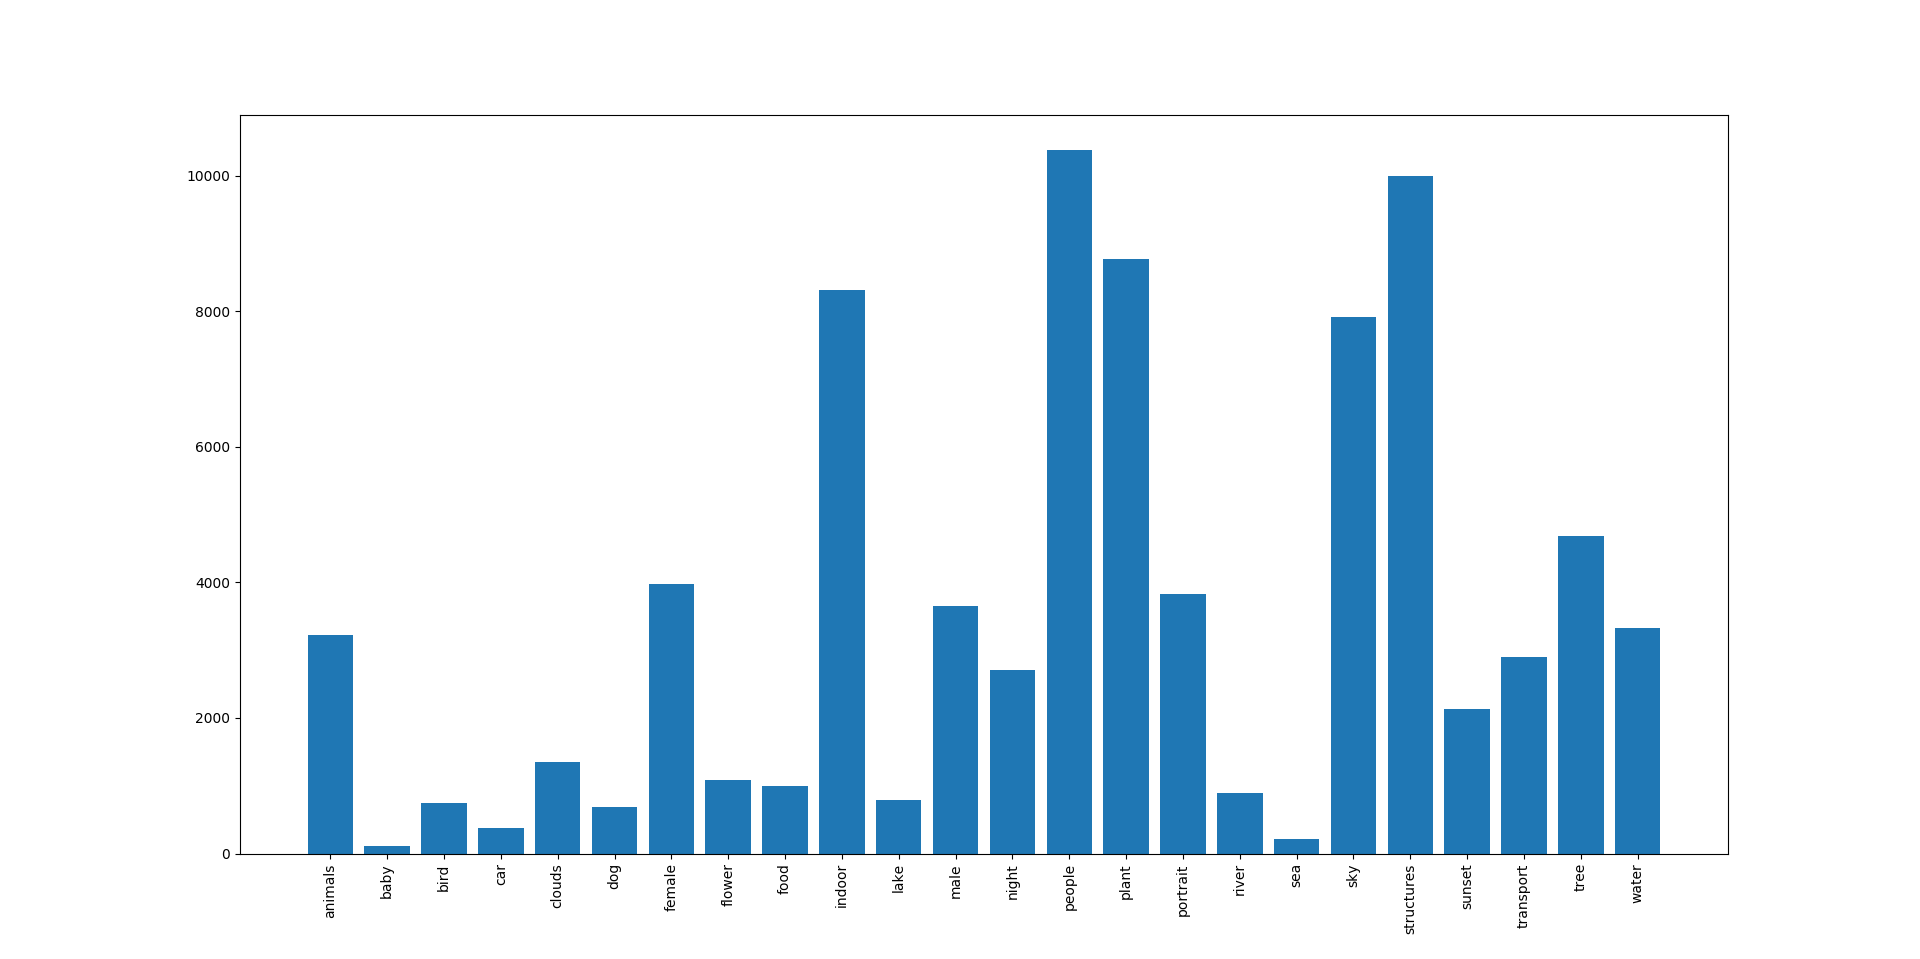
\includegraphics{figs/flikr/classfrequency.png}
		\label{fig:flikr_freq}
		\caption{Number of examples of each class in Flikr25.}
	\end{center}
\end{figure}

\begin{table}[t]
		\centering
		\begin{tabular}{|c|c|}
		\hline
		animals & 3216 \ \hline
		baby & 116 \\ \hline
		bird & 742 \\ \hline
		car & 380 \\ \hline
		clouds & 1350 \\ \hline
		dog & 684 \\ \hline
		female & 3982 \\ \hline
		flower & 1077 \\ \hline
		food & 990 \\ \hline
		indoor & 8313 \\ \hline
		lake & 791 \\ \hline
		male & 3647 \\ \hline
		night & 2711 \\ \hline
		people & 10373 \\ \hline
		plant & 8763 \\ \hline
		portrait & 3829 \\ \hline
		river & 894 \\ \hline
		sea & 214 \\ \hline
		sky & 7912 \\ \hline
		structures & 9992\ \ \hline
		sunset & 2135 \\ \hline
		transport & 2895 \\ \hline
		tree & 4683 \\ \hline
		water & 3331 \\ \hline

		\end{tabular}
		\caption{Number of examples of each class in Flikr25.}
		\label{tab:flikr_freq}
\end{table}

The dataset is randomly split into three sets, a train set, validation set and test set. $\frac{3}{4}$ of the data is used for training, $\frac{1}{16}$ for validation and $\frac{15}{16}$ for testing.	


\subsection{Problem Description}
\subsection{Network Description}
\begin{table}[t]
		\centering
		\begin{tabular}{|c|c|c|c|c|c|c|}
			\hline
			Block & Layer & Type & Neurons & Kernel & Strides & Activation  \\ \hline
			\multirow{4}{*}{Encoder} & 1	&	2D Conv & 32 & (3,3) & (1,1)  & Relu\\ \cline{2-7}
			& 2	&	2D Conv & 64 & (3,3) & (2,2) & Relu \\ \cline{2-7}
			& 3	&	2D Conv & 64 & (3,3) & (2,2) & Relu \\ \cline{2-7}
			& 4 	&	Dropout p=0.25 &	 & 	     &       & \\ \hline
			Embedding & 5	&	2D Conv & 32 & (3,3) & (1,1) & Relu \\ \hline
			Classifier & 6c	&	Dense          & 10 &       &       & Softmax      \\ \hline
			\multirow{5}{*}{Decoder}& 6 	&	Dropout p=0.25 &	 & 	     &       & \\ \cline{2-7}
			& 7	&	2D Trans Convn & 64 & (3,3) & (2,2) & TanH \\ \cline{2-7}
			& 8	&	2D Transp Conv & 64 & (3,3) & (2,2) & TanH \\ \cline{2-7}
			& 9	&	2D Trans Conv & 32 & (3,3) & (1,1) & TanH \\ \cline{2-7}
			& 10	&	2D Trans Conv & 1 & (3,3) & (1,1) & Sigmoid \\ \hline
		\end{tabular}
		\caption{Image classifier. Layer 6c performs classification, whilst the branch starting at layer 6 regenerates the image.}
		\label{tab:flikr_im_description}
	\end{table}
	
\subsection{Results}
\begin{table}
	\centering
		\begin{tabular}{|c|c|c|c|}
		\hline
		Model	& Test Condition & MSE & Acc \\ \hline
		Image	& Im & 	2.2575	&	0.2969 \\ \hline		
		TAG		& Tag & 3.1200	&	0.2196 \\ \hline		
\multirow{3}{*}{Multimodal} & Bi & 2.8306	&	\textbf{0.3182} \\ \cline{2-4}
				& Im & 2.3816	&	0.2530\\ \cline{2-4}	
		
				& Tag & 4.7783	&	0.2304 \\ \hline		
						
		\end{tabular}
		\caption{Results from the combined MNIST Handwritten Digits and UCU Arabic Spoken Digits for the bimodal only testing condition.}
		\label{tab:flikr_res}

\end{table}


%\pgfplotstableread{inputdata.txt}\mydata;
%
%\pgfplotstableset{create on use/Y/.style={create col/copy column from table={dataB.txt}{0}}
%}
%\begin{tikzpicture}
%\begin{axis}
%\addplot table [y=Y] {dataA.txt};
%\end{axis}
%\end{tikzpicture}

\subsection{Discussion}

